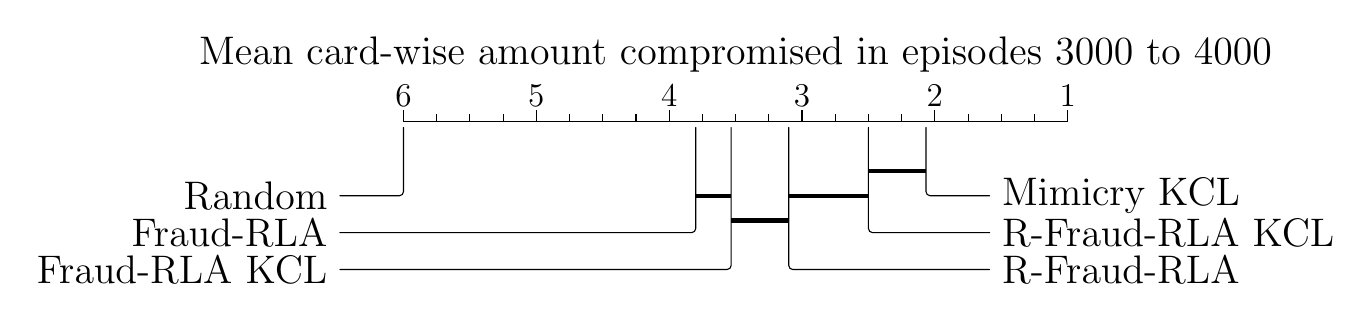
\begin{tikzpicture}[
  treatment line/.style={rounded corners=1.5pt, line cap=round, shorten >=1pt},
  treatment label/.style={font=\Large},
  group line/.style={ultra thick},
]

\begin{axis}[
  clip={false},
  axis x line={center},
  axis y line={none},
  axis line style={-},
  xmin={1},
  ymax={0},
  scale only axis={true},
  width={\axisdefaultwidth},
  ticklabel style={anchor=south, yshift=1*\pgfkeysvalueof{/pgfplots/major tick length}, font=\large},
  every tick/.style={draw=black},
  major tick style={yshift=.5*\pgfkeysvalueof{/pgfplots/major tick length}},
  minor tick style={yshift=.5*\pgfkeysvalueof{/pgfplots/minor tick length}},
  title style={yshift=0.7\baselineskip, font=\Large},
  xmax={6},
  ymin={-4.5},
  height={5\baselineskip},
  xtick={1,2,3,4,5,6},
  minor x tick num={3},
  x dir={reverse},
  title={Mean card-wise amount compromised in episodes 3000 to 4000},
]

\draw[treatment line] ([yshift=-2pt] axis cs:2.066666666666667, 0) |- (axis cs:1.5666666666666669, -2.0)
  node[treatment label, anchor=west] {Mimicry KCL};
\draw[treatment line] ([yshift=-2pt] axis cs:2.5, 0) |- (axis cs:1.5666666666666669, -3.0)
  node[treatment label, anchor=west] {R-Fraud-RLA KCL};
\draw[treatment line] ([yshift=-2pt] axis cs:3.1, 0) |- (axis cs:1.5666666666666669, -4.0)
  node[treatment label, anchor=west] {R-Fraud-RLA};
\draw[treatment line] ([yshift=-2pt] axis cs:3.533333333333333, 0) |- (axis cs:6.5, -4.0)
  node[treatment label, anchor=east] {Fraud-RLA KCL};
\draw[treatment line] ([yshift=-2pt] axis cs:3.8, 0) |- (axis cs:6.5, -3.0)
  node[treatment label, anchor=east] {Fraud-RLA};
\draw[treatment line] ([yshift=-2pt] axis cs:6.0, 0) |- (axis cs:6.5, -2.0)
  node[treatment label, anchor=east] {Random};
\draw[group line] (axis cs:2.5, -2.0) -- (axis cs:3.1, -2.0);
\draw[group line] (axis cs:3.1, -2.6666666666666665) -- (axis cs:3.533333333333333, -2.6666666666666665);
\draw[group line] (axis cs:2.066666666666667, -1.3333333333333333) -- (axis cs:2.5, -1.3333333333333333);
\draw[group line] (axis cs:3.533333333333333, -2.0) -- (axis cs:3.8, -2.0);

\end{axis}
\end{tikzpicture}